%-------------------------------------------------------------------------------
\chapter{Formulation of Model Predictive Control Problem}
\label{ch.MPC}
%-------------------------------------------------------------------------------
Model predictive control \cite{MacMPC} is a mature and widely used control 
paradigm. Its name points to two important characteristics: this strategy
is based on the knowledge of the model of the underlying process, and the behavior
of the system is predicted over some preview horizon. The goal of \ac{MPC} is to
choose a sequence of control inputs for the system over prediction horizon with
respect to given objective function and constraints. This goal can be informally
interpreted as choosing such control inputs, that do not lead to undesirable 
effects in the future. The problem is resolved periodically in order to 
accommodate for the current situation, the preview window is usually shifted in 
time on each iteration of \ac{MPC}. 

Generation of \ac{CoM} and \ac{ZMP} trajectories using an \ac{MPC} scheme was
proposed in \cite{LIPM-MPC}. This chapter reviews some extensions of the scheme
introduced in \cite{WieberMPC, dimitrov2011sparse}.



%%%%%%%%%%%%%%%%%%%%%%%%%%%%%%%%%%%%%%%%%%%%%%%%%%%%%%%%%%%%%%%%%%%%%%%%%%%%%%%%
%%%%%%%%%%%%%%%%%%%%%%%%%%%%%%%%%%%%%%%%%%%%%%%%%%%%%%%%%%%%%%%%%%%%%%%%%%%%%%%%
%%%%%%%%%%%%%%%%%%%%%%%%%%%%%%%%%%%%%%%%%%%%%%%%%%%%%%%%%%%%%%%%%%%%%%%%%%%%%%%%
\section{Unconstrained Model Predictive Control Formulation}
The original \ac{MPC} problem defined in \cite{LIPM-MPC} has finite horizon, a 
quadratic objective function, and is based on a discrete system~\eqref{eq.system_orig}. 
The objective function penalizes distance from predefined reference points for \ac{ZMP}, 
the change in state and control. Since this formulation has no inequality constraints 
an explicit control law ({\bf linear quadratic regulator}) was obtained.

Consider the unconstrained \ac{MPC} based on the system~\eqref{eq.system_orig}
where the objective function is defined equivalently to the objective function
used in \cite{WieberMPC}.
\begin{equation}\label{eq.opt_simple}
\begin{split}
\minimize{\dddot{\mbm{c}}_0 \dots \dddot{\mbm{c}}_{N-1}; \hat{\mbm{c}}_1 \dots \hat{\mbm{c}}_{N}}
            & \frac{1}{2} \sum_{k=1}^{N}   \norm{ \mbm{C} \hat{\mbm{c}}_{k} - \mbm{z}_k^{ref} }^2_{\mbm{Q}} 
            + \frac{1}{2} \sum_{k=0}^{N-1} \norm{ \dddot{\mbm{c}}_k }^2_{\mbm{P}}\\
\subjectto  & \hat{\mbm{c}}_{k+1} = \mbm{A}\hat{\mbm{c}}_{k}+\mbm{B}\dddot{\mbm{c}}_{k},\\
\end{split}
\end{equation}
where 
$$
\mbm{C} = 
\begin{bmatrix}
    1 & 0 & -h & 0 & 0 & 0\\ 
    0 & 0 & 0  & 1 & 0 & -h\\
\end{bmatrix}.
$$
$N$ is the number of sampling intervals in the preview window, matrices $\mbm{Q}$ 
and $\mbm{P}$ contain gains, $\mbm{z}_k^{ref}$ are reference positions for \ac{ZMP}
at discrete sampling time $k$. The objective function does not penalize the change 
in the state $\hat{\mbm{c}}_{k}$, and penalizes the absolute values of control 
inputs instead of change between subsequent control inputs.


%%%%%%%%%%%%%%%%%%%%%%%%%%%%%%%%%%%%%%%%%%%%%%%%%%%%%%%%%%%%%%%%%%%%%%%%%%%%%%%%
%%%%%%%%%%%%%%%%%%%%%%%%%%%%%%%%%%%%%%%%%%%%%%%%%%%%%%%%%%%%%%%%%%%%%%%%%%%%%%%%
%%%%%%%%%%%%%%%%%%%%%%%%%%%%%%%%%%%%%%%%%%%%%%%%%%%%%%%%%%%%%%%%%%%%%%%%%%%%%%%%
\section{Introducing the Inequality Constraints}\label{sec.ds_constraints}
The authors of \cite{WieberMPC} impose constraints on the position of \ac{ZMP}
in order to keep it within the support area and demonstrate that a robot can cope 
with stronger disturbances in this case. Computation of explicit control law for 
\ac{MPC} with inequality constraints \cite{BemporadConstrLQR} is not possible here, 
since the constraints change on each iteration.

Therefore, the application of MPC requires the solution of a quadratic programming 
problem. The quadratic programming is discussed in \cref{ch.QP}. This section is 
focused on the formulation of \ac{MPC} for \ac{CoM}/\ac{ZMP} trajectory generation 
with inequality constraints on \ac{ZMP} positions. This \ac{MPC} is referred to in 
the thesis as \ac{MPCWMG}.


%%%%%%%%%%%%%%%%%%%%%%%%%%%%%%%%%%%%%%%%%%%%%%%%%%%%%%%%%%%%%%%%%%%%%%%%%%%%%%%%
\subsection{Double Support Constraints}
Note that the support area differs depending on the type of support. \ac{SS} can 
be easily represented by a rectangle, while \ac{DS} in a general case cannot. 
Therefore, we need to find a suitable representation of \ac{DS} constraints.

The support area in \ac{DS} is the convex hull of two adjacent \ac{SS}. When the 
\ac{SS} constraints are rectangular, their convex hull is a polygon as shown in 
\cref{fig.ds_hull}. In this case the constraints for \ac{SS} and \ac{DS} must 
be handled differently. We introduce an approximation of this convex hull by
a sequence of rectangles, as demonstrated in \cref{fig.ds_approx}. This approach
allows to define constraints uniformly, furthermore, it makes possible an 
extension of the \ac{MPCWMG} to perform footstep repositioning to compensate for
disturbances \cite{dimitrov2011walking}.
\begin{figure}[ht]
\begin{minipage}[b]{0.4\linewidth}
    \centerline{%
    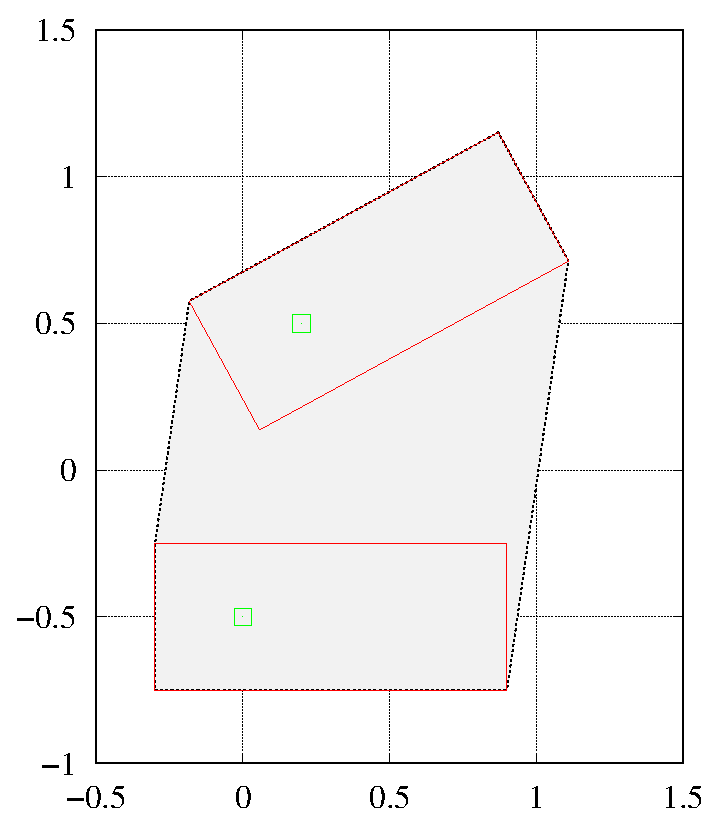
\includegraphics[scale=0.4]{Figures/ds_convex_hull.eps}}
    \caption[Double support]{A double support represented by a convex hull of two single supports}
    \label{fig.ds_hull}
\end{minipage}
\hfill
\begin{minipage}[b]{0.4\linewidth}
    \centerline{%
    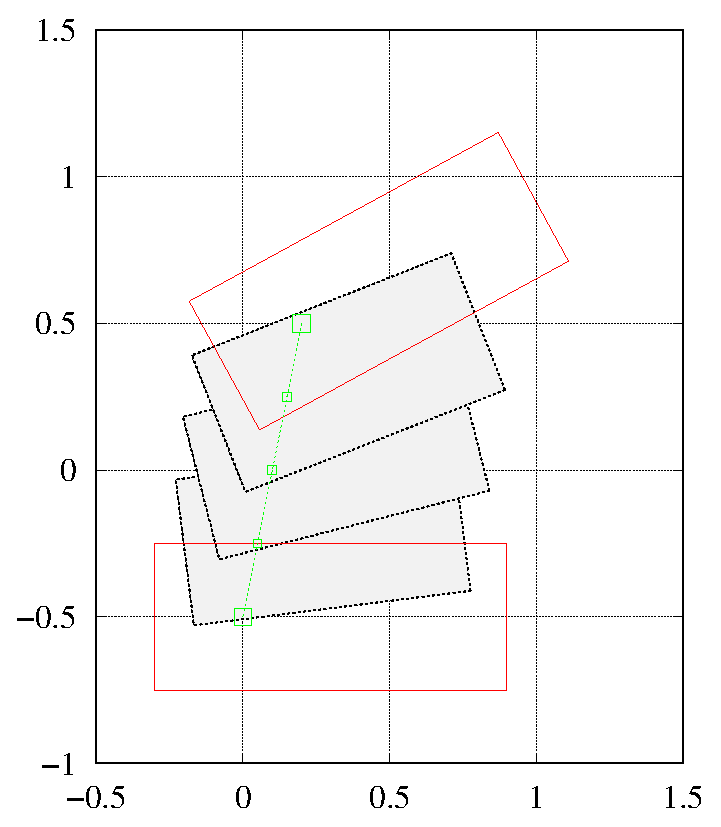
\includegraphics[scale=0.4]{Figures/ds_approx.eps}}
    \caption[Approximate double support]{A double support approximated by a sequence of rectangles}
    \label{fig.ds_approx}
\end{minipage}
\end{figure}


%%%%%%%%%%%%%%%%%%%%%%%%%%%%%%%%%%%%%%%%%%%%%%%%%%%%%%%%%%%%%%%%%%%%%%%%%%%%%%%%
\subsection{Definition of the Inequality Constraints}
A rectangle can be defined with respect to some reference frame $\mathbb{F}$ by
four positive distances 
$\mbm{d} = \begin{bmatrix} u^x & u^y & -l^x & -l^y \end{bmatrix}^T$ 
from the origin of $\mathbb{F}$ to the edges of the rectangle. The position and
orientation of the rectangle are given by the displacement $\mbm{r}$ and angle 
of rotation $\varphi$ of $\mathbb{F}$ with respect to the global reference frame. 
An example is depicted in \cref{fig.constr}.

\begin{figure}[ht]
    \psfragscanon
    \psfrag{r}{$\mbm{r}$}
    \psfrag{a}{$\varphi$}
    \psfrag{h}{$u^x$}
    \psfrag{j}{$u^y$}
    \psfrag{k}{$-l^x$}
    \psfrag{l}{$-l^y$}
    \centerline{%
    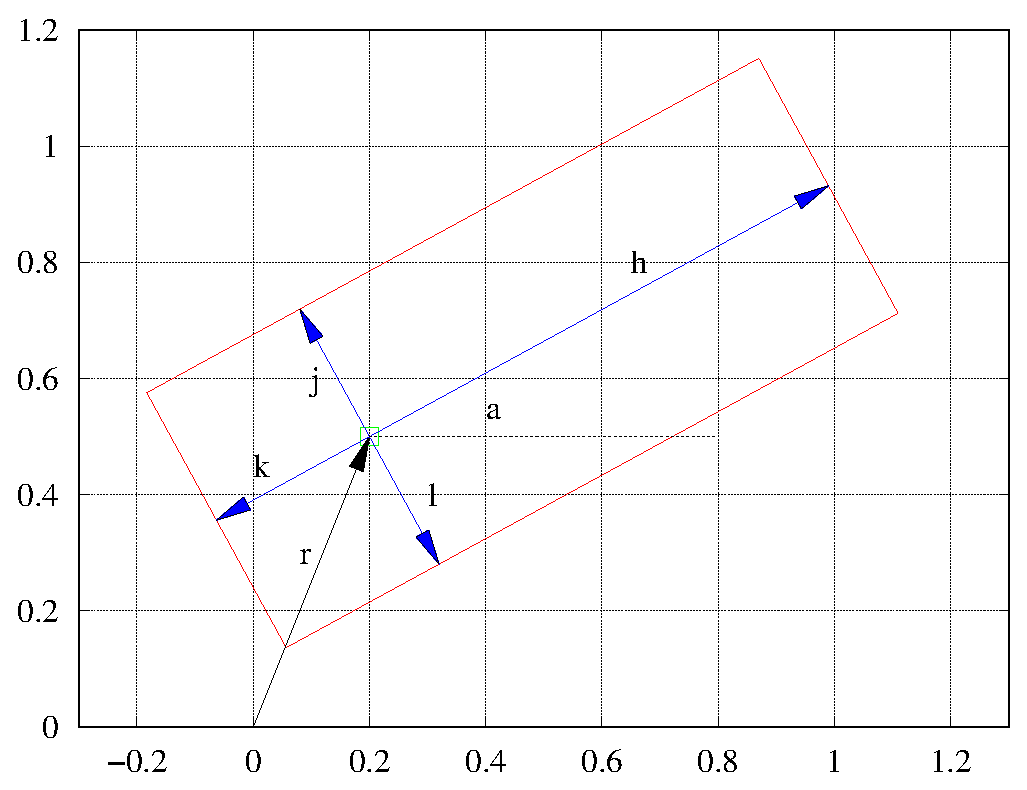
\includegraphics[scale=0.5]{Figures/rect_constraints.eps}}
    \caption[Support rectangle]{Definition of a support rectangle with respect to the global reference frame}
    \label{fig.constr}
\end{figure}

All points $\mbm{p}$ lying within the rectangle satisfy
$$
\mbm{D}\mbm{R}^T\left(\mbm{p} - \mbm{r} \right) \leq \mbm{d},
$$
where matrix $\mbm{D}$ and rotation matrix $\mbm{R}$ are defined as
$$
\mbm{D} = 
\begin{bmatrix}
    \mbm{I}\\
    -\mbm{I}
\end{bmatrix}, \quad
%
\mbm{R} =
\begin{bmatrix}
    \cos\varphi & -\sin\varphi \\
    \sin\varphi & \cos\varphi
\end{bmatrix}.
$$

Thus the constraints for the $k$-th sampling period in the preview window are
\begin{equation}
\mbm{D}\mbm{R}^T_k \mbm{C} \hat{\mbm{c}}_k \leq \mbm{d}_{k} + \mbm{D}\mbm{R}^T_k \mbm{r}_k,
\end{equation}
where 
$$
\mbm{C} = 
\begin{bmatrix}
    1 & 0 & -h & 0 & 0 & 0\\ 
    0 & 0 & 0  & 1 & 0 & -h\\
\end{bmatrix}.
$$
is the output matrix of the system~\ref{eq.system_orig} defined in \cref{sec.3dlipm}.


%%%%%%%%%%%%%%%%%%%%%%%%%%%%%%%%%%%%%%%%%%%%%%%%%%%%%%%%%%%%%%%%%%%%%%%%%%%%%%%%
%%%%%%%%%%%%%%%%%%%%%%%%%%%%%%%%%%%%%%%%%%%%%%%%%%%%%%%%%%%%%%%%%%%%%%%%%%%%%%%%
%%%%%%%%%%%%%%%%%%%%%%%%%%%%%%%%%%%%%%%%%%%%%%%%%%%%%%%%%%%%%%%%%%%%%%%%%%%%%%%%
\section{Time-variant Constrained MPC}\label{sec.timevarsys}
We can exclude the dynamics of the system~\eqref{eq.system_orig} from the inequality 
constraints by replacing the position of the \ac{CoM} by the position of the \ac{ZMP} 
so that
\begin{equation}\label{eq.substitution1}
\tilde{\mbm{c}} = 
\begin{bmatrix} z^x & \dot{c}^x & \ddot{c}^x & z^y & \dot{c}^y & \ddot{c}^y \end{bmatrix}^T,
\end{equation}
to obtain
\begin{equation}\label{eq.constraints}
\mbm{D}\mbm{R}^T_k \mbm{C}_p \tilde{\mbm{c}}_k \leq \mbm{d}_{k} + \mbm{D}\mbm{R}^T_k \mbm{r}_k,
\end{equation}
where
$$
\mbm{C}_p =
\begin{bmatrix}
    1 & 0 & 0 & 0 & 0 & 0 \\
    0 & 0 & 0 & 1 & 0 & 0 \\
\end{bmatrix},
$$

The system must be changed accordingly
\begin{equation}\label{eq.system_sub1}
\tilde{\mbm{c}}_{k+1} = \tilde{\mbm{A}}_k\tilde{\mbm{c}}_{k} + \tilde{\mbm{B}}_k\dddot{\mbm{c}}_{k},
\end{equation}
where the state transition and control matrices are defined as 
$$
\tilde{\mbm{A}}_k =
\begin{bmatrix}
    1 & T_k & \frac{T_k^{2}}{2}-\Delta h_k & 0 & 0 & 0\\ 
    0 & 1 & T_k & 0 & 0 & 0\\ 
    0 & 0 & 1 & 0 & 0 & 0\\
    0 & 0 & 0 & 1 & T_k & \frac{T_k^{2}}{2}-\Delta h_k\\
    0 & 0 & 0 & 0 & 1 & T_k\\
    0 & 0 & 0 & 0 & 0 & 1
\end{bmatrix},
$$
$$
\tilde{\mbm{B}}_k = 
\begin{bmatrix}
    \frac{T_k^{3}}{6} - h_k T_k     & 0\\ 
    \frac{T_k^{2}}{2}               & 0\\ 
    T_k                             & 0\\
    0                               & \frac{T_k^{3}}{6} - h_k T_k\\
    0                               & \frac{T_k^{2}}{2}\\
    0                               & T_k
\end{bmatrix}.
$$
These matrices can be defined as time-invariant, but their parameterization gives us more options 
for tuning. Variation of the \ac{CoM} height during walk, which can be realized through the
appropriate changes of $h_k$, may have a positive effect on the quality of the gait. Also,
the solution of the \ac{QP} may be obtained faster, if the sampling time $T_k$ varies in 
the preview window. Note that the duration of the sampling period in an \ac{MPC} is determined 
by the control sampling time, and all but the first computed control inputs are usually 
discarded. Hence, longer sampling periods in the end of the preview window can be used to 
decrease $N$, which directly affects the time required for solution, without decreasing the 
length of this preview window \cite{dimitrov2008implementation}.

Now we rewrite the optimization problem~\eqref{eq.opt_simple} to reflect the changes 
in the model
\begin{equation}\label{eq.opt}
\begin{split}
\minimize{\dddot{\mbm{c}}_0 \dots \dddot{\mbm{c}}_{N-1}; \tilde{\mbm{c}}_1 \dots \tilde{\mbm{c}}_{N}}
            & \sum_{k=1}^{N}    \norm{ \tilde{\mbm{c}}_k - \mbm{C}_p^T \mbm{z}_k^{ref} }^2_{\tilde{\mbm{Q}}} 
            + \sum_{k=0}^{N-1}  \norm{ \dddot{\mbm{c}}_k }^2_{\mbm{P}}\\ 
\subjectto  & \tilde{\mbm{c}}_{k+1} = \tilde{\mbm{A}}_k\tilde{\mbm{c}}_{k} + \tilde{\mbm{B}}_k\dddot{\mbm{c}}_{k}\\
            & \mbm{D}\mbm{R}^T_k \mbm{C}_p \tilde{\mbm{c}}_k \leq \mbm{d}_{k} + \mbm{D}\mbm{R}^T_k \mbm{r}_k, 
\end{split}
\end{equation}
where the gain matrices are
$$
\tilde{\mbm{Q}} =
\begin{bmatrix}
    \frac{\alpha_g}{2} & 0                 & 0 & 0 & 0 & 0\\ 
    0               & \frac{\beta_g}{2}  & 0 & 0 & 0 & 0\\ 
    0               & 0                 & \frac{\gamma_g}{2} & 0 & 0 & 0\\ 
    0 & 0 & 0 & \frac{\alpha_g}{2} & 0                 & 0 \\ 
    0 & 0 & 0 & 0               & \frac{\beta_g}{2}  & 0 \\ 
    0 & 0 & 0 & 0               & 0                 & \frac{\gamma_g}{2} \\ 
\end{bmatrix}, \quad
\mbm{P} = 
\begin{bmatrix}
      \frac{\eta_g}{2}  & 0  \\ 
      0                 &  \frac{\eta_g}{2} \\ 
\end{bmatrix}.
$$

The first term in the objective function is
\begin{equation*}
\begin{split}
    \sum_{k=1}^{N} \norm{ \tilde{\mbm{c}}_k - \mbm{C}_p^T \mbm{z}_k^{ref} }^2_{\tilde{\mbm{Q}}} &=
    \sum_{k=1}^{N} \left(
        \norm{ \tilde{\mbm{c}}_k }^2_{\tilde{\mbm{Q}}} 
        + \norm{ \mbm{C}_p^T \mbm{z}_k^{ref} }^2_{\tilde{\mbm{Q}}}
        - 2 \tilde{\mbm{c}}_k^T \tilde{\mbm{Q}} \mbm{C}_p^T \mbm{z}_k^{ref}
    \right)\\
    &= \sum_{k=1}^{N} \left(
        \norm{ \tilde{\mbm{c}}_k }^2_{\tilde{\mbm{Q}}} 
        + \norm{ \mbm{C}_p^T \mbm{z}_k^{ref} }^2_{\tilde{\mbm{Q}}}
        - \alpha_g (\mbm{C}_p^T \mbm{z}_k^{ref})^T \tilde{\mbm{c}}_k
    \right)\\
    &= \sum_{k=1}^{N} \left(
        \norm{ \tilde{\mbm{c}}_k }^2_{\tilde{\mbm{Q}}} 
        + \norm{ \mbm{C}_p^T \mbm{z}_k^{ref} }^2_{\tilde{\mbm{Q}}}
        + \mbm{q}_k^T \tilde{\mbm{c}}_k
    \right),
\end{split}
\end{equation*}
where $\mbm{q}_k = - \alpha_g (\mbm{C}_p^T \mbm{z}_k^{ref})$.

The terms $\norm{ \mbm{C}_p^T \mbm{z}_k^{ref} }^2_{\tilde{\mbm{Q}}}$ are constant
and can be dropped. Thus we obtain the following formulation \ac{MPCWMG}
\begin{equation}\label{eq.opt_final}
\begin{split}
\minimize{\dddot{\mbm{c}}_0 \dots \dddot{\mbm{c}}_{N-1}; \tilde{\mbm{c}}_1 \dots \tilde{\mbm{c}}_{N}}
            & \sum_{k=1}^{N}    \norm{ \tilde{\mbm{c}}_k }^2_{\tilde{\mbm{Q}}} 
            + \sum_{k=0}^{N-1}  \norm{ \dddot{\mbm{c}}_k }^2_{\mbm{P}} 
            + \sum_{k=1}^{N}    \mbm{q}_k^T \tilde{\mbm{c}}_k\\
\subjectto  & \tilde{\mbm{c}}_{k+1} = \tilde{\mbm{A}}_k\tilde{\mbm{c}}_{k} + \tilde{\mbm{B}}_k\dddot{\mbm{c}}_{k}\\
            & \mbm{D}\mbm{R}^T_k \mbm{C}_p \tilde{\mbm{c}}_k \leq \mbm{d}_{k} + \mbm{D}\mbm{R}^T_k \mbm{r}_k.
\end{split}
\end{equation}


%%%%%%%%%%%%%%%%%%%%%%%%%%%%%%%%%%%%%%%%%%%%%%%%%%%%%%%%%%%%%%%%%%%%%%%%%%%%%%%%
%%%%%%%%%%%%%%%%%%%%%%%%%%%%%%%%%%%%%%%%%%%%%%%%%%%%%%%%%%%%%%%%%%%%%%%%%%%%%%%%
%%%%%%%%%%%%%%%%%%%%%%%%%%%%%%%%%%%%%%%%%%%%%%%%%%%%%%%%%%%%%%%%%%%%%%%%%%%%%%%%
\section{Generation of an Initial Guess}\label{sec.init_guess}
The \ac{MPC} problem~\eqref{eq.opt_final} is always feasible. This is a useful
property for generation of an initial feasible point.

At each iteration of \ac{MPCWMG} the current state of the system~\eqref{eq.system_sub1}
is assumed to be known. It is also possible to find a set of $N$ points satisfying the
inequality constraints~\eqref{eq.constraints} for each sampling period. This
set is a feasible profile for \ac{ZMP}, the next step is to generate control inputs 
to follow this profile and determine the unknown state variables using a simple
iterative procedure.

The $k$-th control inputs can be computed based on the current state and the next 
\ac{ZMP} position by multiplying both sides of \cref{eq.system_sub1} by $\mbm{C}_p$
$$
\dddot{\mbm{c}}_{k} = (\mbm{C}_p\tilde{\mbm{B}}_k)^{-1} (\mbm{z}_{k+1} 
                    - \mbm{C}_p \tilde{\mbm{A}}_k\tilde{\mbm{c}}_{k}).
$$
Matrix $\mbm{C}_p\tilde{\mbm{B}}_k$ is not invertible when $c^z_k = T_k^2 / 6$.
If the sampling period is less than $0.1$ second, then the height of \ac{CoM} 
of a robot must be lower than approximately $2$ millimeters in order to satisfy 
this equality. Since the sampling period used in simulations and experiments is 
always below $0.1$ second, it is safe to assume that the matrix is always invertible.

Having the $k$-th control inputs and the current state it is possible to find 
velocity and acceleration of the next state using \cref{eq.system_sub1}.


%%%%%%%%%%%%%%%%%%%%%%%%%%%%%%%%%%%%%%%%%%%%%%%%%%%%%%%%%%%%%%%%%%%%%%%%%%%%%%%%
%%%%%%%%%%%%%%%%%%%%%%%%%%%%%%%%%%%%%%%%%%%%%%%%%%%%%%%%%%%%%%%%%%%%%%%%%%%%%%%%
%%%%%%%%%%%%%%%%%%%%%%%%%%%%%%%%%%%%%%%%%%%%%%%%%%%%%%%%%%%%%%%%%%%%%%%%%%%%%%%%
\section{Stability of the MPC scheme}\label{sec.mpc_stability}
When an \ac{MPC} with finite horizon is used, its stability must be considered.
It is possible to ensure stability using appropriate modifications of the problem,
for a comprehensive review refer to \cite{MPCstab}. Stability of the \ac{MPC} 
formulations presented so far is not guaranteed. Moreover, it is difficult to
judge on the stability of the \ac{MPCWMG}, since the problem is altered on each 
iteration due to the change of the set of the inequality constraints.

Let us neglect the changes of the constraints for the moment and consider the 
\ac{QP} problem, which is solved on a particular iteration. Note that the discrete 
systems~\eqref{eq.system_orig} and~\eqref{eq.system_sub1} are unstable, since the 
state transition matrices have repeated eigenvalues equal to $1$ and the dimesion 
of the respective Jordan blocks is greater than $1$. Consequently, it is necessary to 
impose terminal constraints in order to ensure stability \cite{MuskeLinearMPC}. 
\ac{QP} with terminal constraints may become infeasible, and generation of an initial 
guess (\cref{sec.init_guess}) may become more computationally expensive. The stable 
\ac{MPCWMG} may improve the ability of a robot to cope with external disturbances 
and may require shorter preview window. However, the effect on the quality of the 
gait is unknown. Furthermore, the stability of \ac{MPCWMG} does not imply, that the 
generated \ac{CoM} trajectory can be executed by the controlled robot. Hence, the 
stability of the \ac{MPCWMG} scheme requires special consideration and experiments, 
and it was decided to leave it out of the scope of the thesis.

In order to avoid stability issues a ``sufficiently long'' preview window is
used. In \cite{LIPM-MPC}, where \ac{MPC} problem is not constrained, the explicit 
control law was computed, and the preview gain was shown to be decreasing to a very
small value in about $2$ seconds. The built-in walking module for Nao uses preview 
window of $0.8$ second \cite{NaoWalk}. In a similar way, the necessary preview window 
length for the developed walking module was found experimentally (it is about $1.6$ 
second, see \cref{ch.results}). Since this time is related to the speed of walk, 
the number of footsteps is likely to be a better measure of a preview horizon. In our 
implementation $1.6$ second includes three \ac{SS}, or one full oscillation of the 
\ac{ZMP} trajectory.

% {\bf robust} \ac{MPC} and {\bf stochastic} \ac{MPC}
%orbital stability
%constraints on z vs c cddot
%\cite{RaoIPMPC}
